\section{Can an AI tell it has never heard this before?}
\label{sec:novelty}

\begin{figure*}[t]
\centering
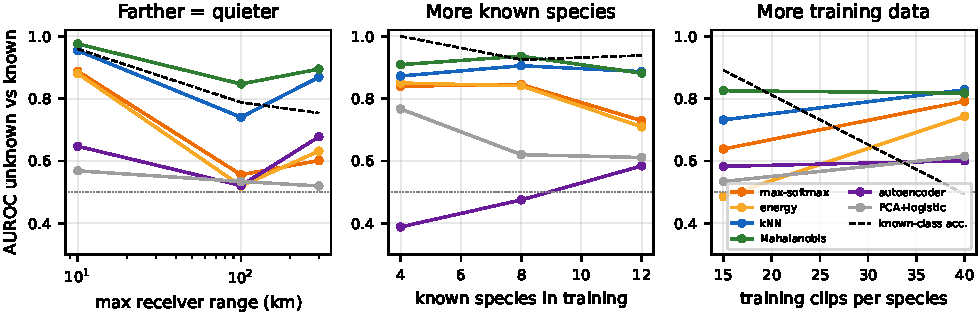
\includegraphics[width=\textwidth]{figures/novelty_sweeps.pdf}
\caption{AUROC of six novelty scores (unknown vs known species) on the
synthetic soundscape as the receiver range grows (left; farther means lower
SNR), as the number of known species grows (middle) and as training clips per
species grow (right). The dashed line is the closed-set accuracy on known
species.}
\label{fig:sweeps}
\end{figure*}

\paragraph{Synthetic soundscape.} On the base condition
(Figure~\ref{fig:sweeps}, and the blue bars of Figure~\ref{fig:real}) the CNN
reaches \NovAccBase\ closed-set accuracy, and the embedding-space scores
separate unknown species from known ones with AUROC \NovAurocKnn\ (kNN, 95\%
bootstrap CI \NovBestCiLo--\NovBestCiHi) and \NovAurocMaha\ (Mahalanobis),
against \NovAurocMsp\ for max-softmax, \NovAurocEnergy\ for energy,
\NovAurocAe\ for the autoencoder and \NovAurocPcamsp\ for the PCA baseline.
The ordering is the one reported on image benchmarks: the geometry of the
embedding knows more about novelty than the confidence of the head, and a
reconstruction error trained only on known clips barely beats chance (best
\NovAeMax\ across conditions) because a new call is still a call and
reconstructs well. Even the best score has a false-positive rate of
\NovBestFpr\% at 95\% recall of unknowns, which is why the flagging step
below uses a high threshold and expects to miss some novel clips.

\paragraph{Range and data.} Novelty degrades gracefully with distance: from a
10\,km ceiling (SNR \NovSnrNear\,dB) to 300\,km (\NovSnrFar\,dB), Mahalanobis
falls from \NovMahaNear\ to \NovMahaFar\ and kNN to \NovKnnFar, while
max-softmax drops from \NovMspNear\ to \NovMspFar. With only four known species
the Mahalanobis score is still \NovMahaFour\ (max-softmax \NovMspFour), and
with 15 training clips per species \NovMahaClipsFifteen\ (max-softmax
\NovMspClipsFifteen): the distance-based scores are robust to small
catalogues, the confidence-based ones are not, and for deep-sea work the
catalogue \emph{is} small.

\begin{figure}[t]
\centering
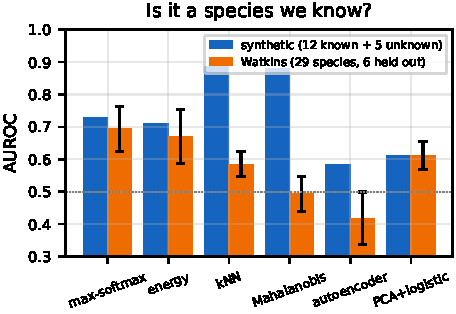
\includegraphics[width=\columnwidth]{figures/novelty_real.pdf}
\caption{Novelty AUROC per score on the synthetic soundscape (base
condition), on real Watkins calls with a from-scratch CNN, and on the same
real clips with a frozen pretrained backbone (AST) in place of the CNN
(\RealSpecies\ species, \RealNUnknown\ held out as unknown, mean $\pm$
s.d.\ over 10 holdout draws).}
\label{fig:real}
\end{figure}

\paragraph{Real calls, from-scratch CNN.} The orange bars of
Figure~\ref{fig:real} are the honest part. A CNN trained from scratch on
\RealClips\ clips reaches only \RealAcc\ closed-set accuracy on
\RealSpecies\ species, and the best novelty score is \RealBestScore\ at
AUROC \RealBestAuroc; the embedding-space scores that dominate on
synthetic data fall to \RealAurocKnn\ (kNN) and \RealAurocMaha\
(Mahalanobis), i.e.\ the embedding has not learned species geometry. Real
recordings vary in recorder, distance, background and duration far more
than our simulator.

\paragraph{Real calls, pretrained backbone.} The green bars swap the
from-scratch CNN for a frozen Audio Spectrogram Transformer embedding
(\texttt{\RealPtBackbone}), with no
fine-tuning, feeding the same six scores through a deterministic
sklearn probe instead of a second from-scratch classifier. Accuracy rises
to \RealPtAcc\ and the best score to \RealPtBestAuroc\ (\RealPtBestScore),
a paired improvement of $\Delta=$\RealPtDelta\ that is positive in every
one of the 10 holdout draws. This confirms the diagnosis directly: the
embedding, not the scoring method, was the bottleneck on real data, and
the fix is a frozen off-the-shelf model, not more deep-sea recordings
(which do not exist at the scale a from-scratch embedding would need).

\begin{figure*}[t]
\centering
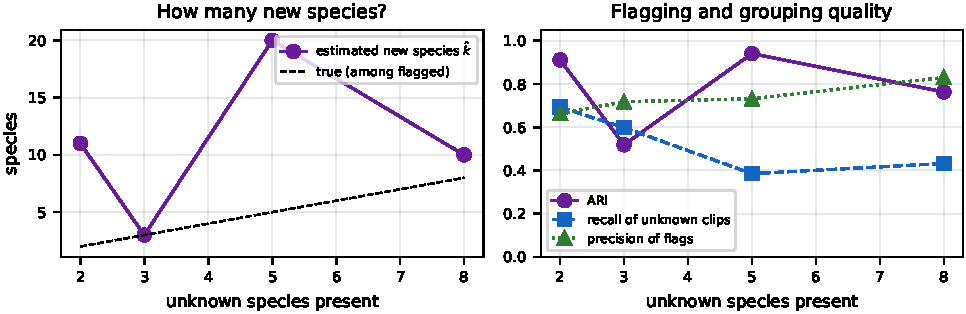
\includegraphics[width=\textwidth]{figures/cluster.pdf}
\caption{Clustering the flagged clips. Left: estimated number of new species
(silhouette-selected $\hat k$) versus the number of unknown species actually
present among the flagged clips. Right: adjusted Rand index of the clusters
against the true unknown species, and the recall and precision of the
flagging step.}
\label{fig:cluster}
\end{figure*}

\paragraph{How many new species?} Figure~\ref{fig:cluster} takes the flagged
clips (precision $\geq$ \CluPrecMin\ at every $U$, recall \CluRecallUTwo--\CluRecallUFive)
and asks whether they group into the unknown species. With two or three
unknown species the clusters are nearly perfect (ARI \CluAriUTwo\ and
\CluAriUThree), though the silhouette criterion over-splits to
$\hat k = \CluKhatUTwo$; with five or eight unknown species the silhouette
prefers two or three broad clusters (ARI \CluAriUFive, \CluAriUEight) ---
it groups the novel clips by call family rather than by species. This is the
step where a human (or a second, finer model) enters: the system reliably
says ``here are the clips that are not in the catalogue, and they come in a
few kinds''; counting the kinds precisely needs either better embeddings or
the taxonomist. On real data the same procedure gives a mean ARI of
\RealAriMean, consistent with the weak embedding.
